\documentclass[a0,portrait]{sciposter}

\usepackage[utf8]{inputenc}

\usepackage{amsmath,bm,bbm} 
\usepackage{url}     
\usepackage{enumitem}
\usepackage{blindtext}
\usepackage{bbding}
\usepackage{multicol} % This is so we can have multiple columns of text side-by-side
\columnsep=100pt % This is the amount of white space between the columns in the poster
\columnseprule=3pt % This is the thickness of the black line between the columns in the poster
\usepackage[portuguese,activeacute]{babel}
\usepackage{babelbib}
\usepackage[svgnames]{xcolor} % Specify colors by their 'svgnames', for a full list of all colors available see here: http://www.latextemplates.com/svgnames-colors
\usepackage{times} % Use the times font
%\usepackage{palatino} % Uncomment to use the Palatino font
\usepackage{amsmath}
\usepackage{graphicx} % Required for including images
\graphicspath{{figures/}} % Location of the graphics files
\usepackage{booktabs} % Top and bottom rules for table
\usepackage[font=small,labelfont=bf]{caption} % Required for specifying captions to tables and figures
\usepackage{amsfonts, amsmath, amsthm, amssymb} % For math fonts, symbols and environments
\usepackage{wrapfig} % Allows wrapping text around tables and figures


\title{\Huge \textcolor{black}{Análise de Sinais com Distâncias Estocásticas e Diferenças de Entropias - Ferramentas para Análise de Séries Temporais}}
\author{Eduarda T.\ C.\ Chagas$^{1}$, Alejandro C.\ Frery$^{2}$}
\institute{$^{1}$Estudante de IC de Ciência da Computação, Ufal\\
$^{2}$Pesquisador do LaCCAN, Ufal}
\email{1.03.02 - Ciência da Computação / Matemática da Computação}
\conference{\textcolor{black}{{\bf SBPC 2018} --
1.03.02 - Ciência da Computação / Matemática da Computação}}

\leftlogo[1.5]{laccan}
%\rightlogo[.6]{ufal.png}
\rightlogo{sbpc.jpg}

\begin{document}

\maketitle

\vspace{1cm}

\begin{multicols}{2} % This is how many columns your poster will be broken into, a portrait poster is generally split into 2 columns

%----------------------------------------------------------------------------------------
%	INTRODUCTION
%----------------------------------------------------------------------------------------

\color{Black}
\section*{Introdução}

\quad Séries temporais são conjunto de dados obtidos a partir de um processo observacional ao longo de um determinado período de tempo, não necessariamente dividido em espaços iguais, sendo caracterizadas pela dependência serial existente entre as observações.\\

O projeto aqui relatado tomou como ponto de partida a identificação das necessidades dos pesquisadores: uma ferramenta gráfica amigável e funcionalidades rápidas, eficientes e numericamente confiáveis para a aplicação de técnicas não paramétricas à análise de séries temporais.
Outro requisito foi o da portabilidade para diversos sistemas operacionais e arquiteturas de hardware, e o uso de ferramentas FLOSS (\textit{Free/Libre Open Source Software}).\\
 
Apresentamos, assim, o desenvolvimento de uma ferramenta portável, rápida e de boa qualidade numérica que possibilita análises interativas e exploratórias dos dados de uma série temporal através de técnicas provenientes da Teoria da Informação.
Com ela, o usuário dispõe de uma conjunto técnicas de análise presentes na literatura para processar e examinar seus dados de modo eficiente e com um mínimo período de aprendizado.
A ferramenta é extensível.\\

\textbf{Palavras-chave:} Teoria da Informação, plataforma \texttt R, Estatística Computacional.

\textbf{Apoio financeiro:} CNPq (Conselho Nacional de Desenvolvimento Científico e \\Tecnológico).

\section*{Metodologia}.

\quad A primeira parte do projeto consistiu da apropriação do referencial teórico.
Seja a série temporal $\bm x = (x_1, x_2, \dots, x_n)$.
Ao invés de analisarmos os valores, transformaremos grupos de $N$ valores (não necessariamente adjacentes) e padrões ordinais, e analisaremos a sua distribuição de frequência.
Por exemplo e sem perda de generalidade, com $N=3$ e para qualquer $i$ viável,
se $x_i<x_{i+1}<x_{i+2}$ assignaremos a esta tripla o padrão $\pi_0$;
caso $x_i>x_{i+1}>x_{i+2}$ o padrão será $\pi_1$ e assim por diante.
Com isso, há $N!$ possíveis padrões.
Esta é conhecida como \textit{simbolização de Bandt \& Pompe}~\cite{PermutationEntropyBandtPompe}.\\

Forma-se, então, um histograma e, a partir dele, extraem-se quantificadores como, por exemplo, entropia, distância estocástica a uma distribuição de equilíbrio, e complexidade estatística.\\

Seja, assim, $\bm h=(h_1,\dots,h_{N!})$ o histograma de proporções dos $N!$ padrões observados a partir da série temporal $\bm x$.
Calculamos a entropia de Shannon

\begin{equation}
H(\bm h) = \sum_{i=1}^{N!} (-\log h_i) h_i,
\label{eq:Entropia}
\end{equation}

A entropia de Shannon é o primeiro elemento a descrever a nossa série temporal.
Ela mede a desordem do sistema que deu origem aos dados $\bm x$.\\

Calculamos logo a distância de Jensen-Shannoon à distribuição uniforme $\bm u=(1/N!,\dots,1/N!)$
\begin{equation}
D(\bm h,\bm u) = \sum_{i=1}^{N!} \Big(h_i \log\frac{h_i}{u_i} +
u_i \log\frac{u_i}{p_i}
\Big),
\end{equation}

em que $u_i=1/N!$
Esta é uma medida de quão perto ou longe a dinâmica subjacente está de um processo sem informação nenhuma.\\

Finalmente, calculamos o terceiro descritor da nossa série temporal: a sua Complexidade Estatística:

\begin{equation}
C(\bm h, \bm u) = H(\bm h) D(\bm h, \bm u).
\end{equation}

Cada série temporal pode então ser descrita por um ponto $(H(\bm h), C(\bm h, \bm u))$.
O conjunto de todos os pares $(H(\bm h), C(\bm h, \bm u))$ para qualquer série temporal descrita por padrões de comprimento $N$ jaz em um subconjunto compacto $\mathbbm R^2$: o plano Entropia-Complexidade.\\

Embora aqui relatemos apenas o uso da entropia de Shannon e da distância de Jensen-Shannon, o sistema oferece outras entropias~\cite{salicruetal1993} e distâncias estocásticas~\cite{StatisticalInferenceBasedonDivergenceMeasures}.

%----------------------------------------------------------------------------------------
%	RESULTADOS E DISCUSSÕES
%----------------------------------------------------------------------------------------

\section*{Resultados e discussões}
\quad Seguindo o modelo de engenharia de software em espiral, o sistema foi projetado e desenvolvido de forma modular, composto pelas seguintes unidades:

\begin{itemize}[leftmargin=1.0in]
\item Módulo de simbolização;
\item Módulo de análise;
\item Modulo de visualização e interação (em fase de desenvolvimento);
\end{itemize} 

Esses módulos foram e estão sendo desenvolvidos seguindo um cronograma. Depois passaram pelas seguintes etapas:
\begin{enumerate}[leftmargin=1.0in]
\item Integração dos módulos em um sistema;
\item Teste e validação do sistema (em fase de desenvolvimento);
\item Geração da interface gráfica (em fase de desenvolvimento).
\end{enumerate}

Permite-se a leitura de dados em vários formatos (TXT, CSV ou XLSX), e o usuário a seguir poderá escolher:

\begin{itemize}[leftmargin=1.0in]
	\item[\HandRight] Gerar o gráfico da série;
	\item[\HandRight] Calcular seus diversos valores de Entropia;
	\item[\HandRight] Calcular seus diversos valores de Distâncias estocásticas;
	\item[\HandRight] Calcular complexidades estatísticas;
    \item[\HandRight] Identificar padrões no gráfico da série temporal;
    \item[\HandRight] Gerar planos de Entropias;
    \item[\HandRight] Gerar planos de Distâncias estocásticas;
	\item[\HandRight] Gerar o histograma de padrões;
	\item[\HandRight] Identificar o ponto característico da série no plano Entropia-Complexidade.
\end{itemize}

Um elemento original do sistema é a vinculação entre o histograma de padrões e a série temporal. Escolhendo um ou mais elementos do histograma, os valores correspondentes na série temporal aparecem realçados.

\begin{center}\vspace{1cm}
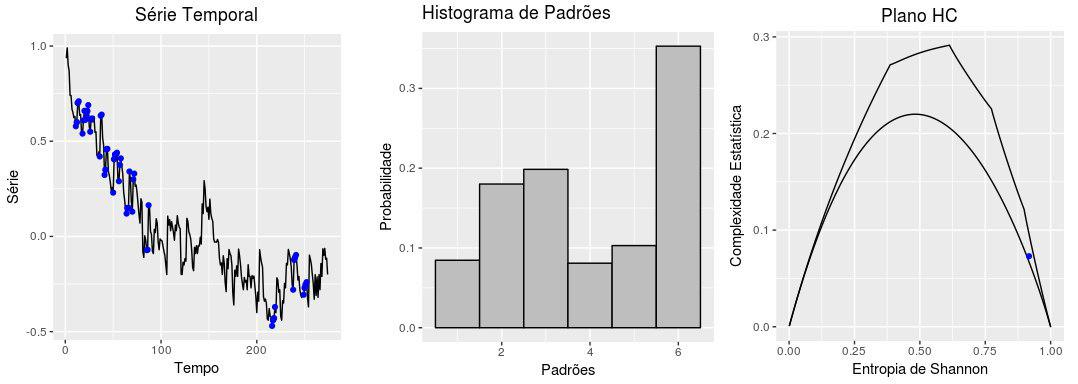
\includegraphics[width=1\linewidth]{img1}
\captionof{figure}{A figura acima ilustra o processo de extração de informações de uma série temporal que representa anomalias médias globais da temperatura em graus Celsius em relação a um período base (GISTEMP e GCAG).  Os dados se encontram disponíveis em \url{https://pkgstore.datahub.io/core/global-temp/annual_csv/data/a26b154688b061cdd04f1df36e4408be/annual_csv.csv}. A imagem 1.1 nos informa a presença dos padrões $(2,0,1)$ na série. Já a imagem 1.2 apresenta o histograma de densidade, utilizado posteriormente como função de probabilidade. Por último, a figura 1.3 no mostra a representação de tais dados no Plano HC}
\end{center}\vspace{1cm}

%----------------------------------------------------------------------------------------
%	CONCLUSÕES
%----------------------------------------------------------------------------------------

\section*{Conclusões}

\quad Através do desenvolvimento deste projeto realizamos o desenvolvimento de uma ferramenta portável, rápida e de boa qualidade numérica que possibilita análises interativas e exploratórias dos dados de uma série temporal através de técnicas provenientes da Teoria da Informação.
Por meio desta, o usuário tem acesso a um conjunto técnicas de análise presentes na literatura para processar e examinar seus dados, realizando isto em um mínimo período de aprendizado.

%----------------------------------------------------------------------------------------
%	REFERENCES
%----------------------------------------------------------------------------------------

\nocite{*}
\bibliographystyle{plain} 
\bibliography{ref} 



\end{multicols}
\end{document}